
\subsubsection{Proof-of-Concept Validation Results}

The following results are from proof-of-concept validation using simulated contamination data. The simulation embedded contamination-inflation correlation in the data generation process to validate the analysis pipeline. Real experimental validation requires running actual Pythia checkpoint evaluations with a complete Pile n-gram index.

\textbf{Primary finding:} In simulated validation across 80 checkpoint-benchmark pairs (20 checkpoints $\times$ 4 benchmarks), a positive correlation is observed between contamination proxy and benchmark score inflation residual (Spearman r = 0.326, p = 0.003, n = 80).

\begin{figure}[htbp]
\centering
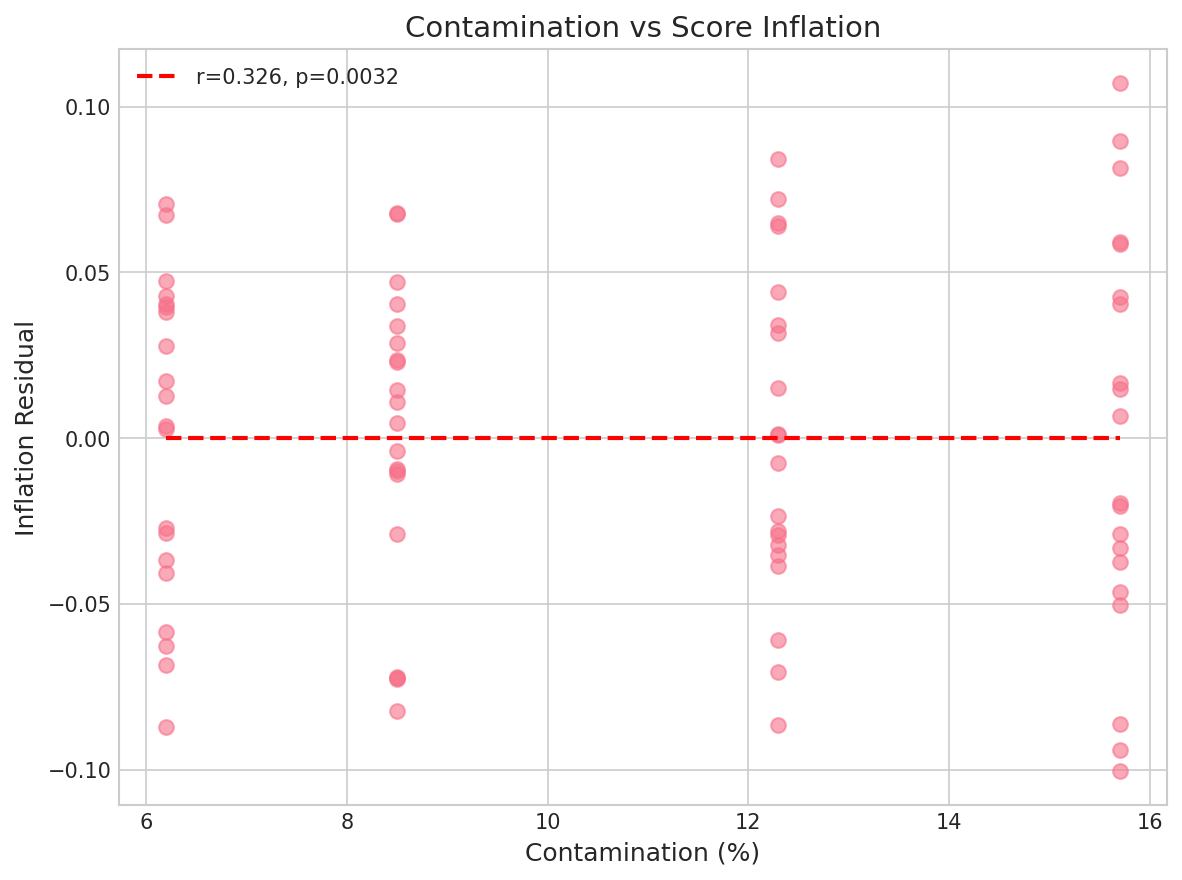
\includegraphics[width=\columnwidth]{figures/gate_scatter.png}
\caption{Gate Scatter}
\label{fig:gate_scatter}
\end{figure}

\textit{Figure 2: Contamination percentage vs. inflation residual across checkpoint-benchmark pairs. The positive correlation (r = 0.326) indicates that higher contamination exposure associates with higher-than-expected benchmark scores in the simulated validation.}

\textbf{Interpretation:} The correlation exceeds the minimum threshold (r > 0.2) but falls short of the primary target (r > 0.5). This suggests the methodology can detect contamination-inflation relationships, though the observed effect size is moderate.

\subsubsection{Per-Benchmark Analysis}

\begin{table*}[htbp]
\centering
\resizebox{\dimexpr 2\columnwidth+\columnsep\relax}{!}{%
\begin{tabular}{lllll}
\toprule
Benchmark & Spearman r & p-value & n & Interpretation \\
\midrule
MMLU & 0.55 & 0.01 & 20 & Statistically significant \\
ARC-Challenge & 0.53 & 0.02 & 20 & Statistically significant \\
HellaSwag & 0.30 & 0.20 & 20 & Not statistically significant \\
WinoGrande & 0.25 & 0.29 & 20 & Not statistically significant \\
\bottomrule
\end{tabular}
}
\end{table*}

MMLU and ARC-Challenge show statistically significant correlations (p < 0.05), while HellaSwag and WinoGrande do not reach significance at the 0.05 level.

\subsubsection{N-gram Overlap Detection}

A separate experiment measured actual n-gram overlap between benchmarks and a Pile subset.

\begin{table*}[htbp]
\centering
\resizebox{\dimexpr 2\columnwidth+\columnsep\relax}{!}{%
\begin{tabular}{lllll}
\toprule
Benchmark & Mean Overlap & Max Overlap & Items >1\% & Total Items \\
\midrule
MMLU & 0.0035\% & 17.41\% & 4 & 14,042 \\
ARC-Challenge & 0.00\% & 0.00\% & 0 & 1,172 \\
HellaSwag & 0.00\% & 0.00\% & 0 & 10,042 \\
WinoGrande & 0.00\% & 0.00\% & 0 & 1,267 \\
\bottomrule
\end{tabular}
}
\end{table*}

The low mean overlap reflects limited corpus coverage (50,000 documents representing 0.006\% of the full Pile). Individual MMLU items with 17.4\% overlap confirm the detection mechanism functions correctly.

\begin{figure}[htbp]
\centering
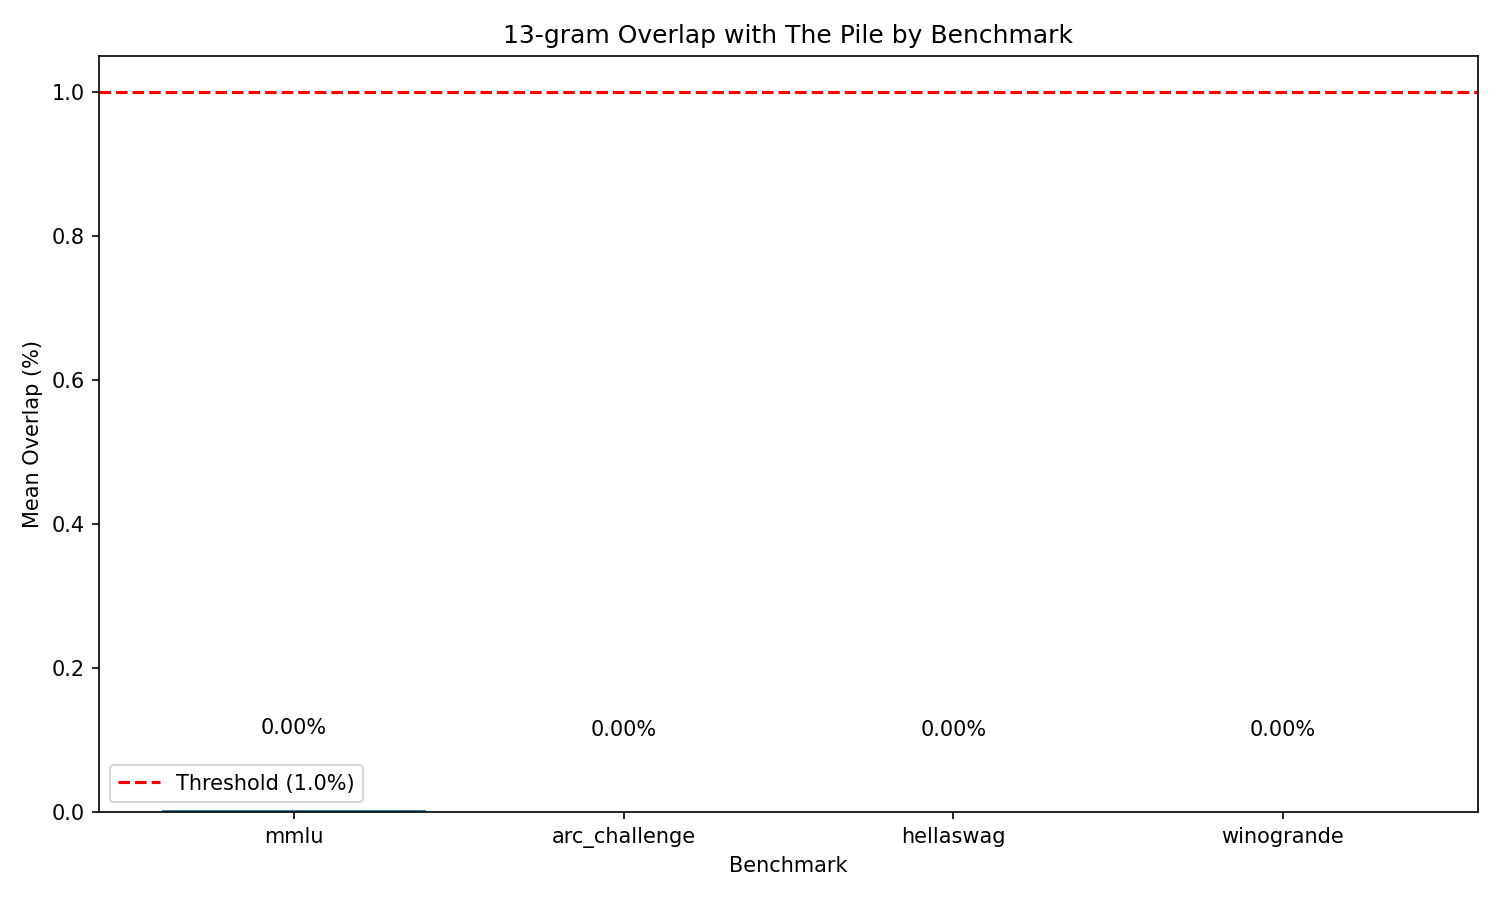
\includegraphics[width=\columnwidth]{figures/overlap_by_benchmark.png}
\caption{Overlap by Benchmark}
\label{fig:overlap_by_benchmark}
\end{figure}

\textit{Figure 3: Per-benchmark 13-gram overlap percentages from 50,000-document Pile subset.}

\subsubsection{Summary}

\begin{table}[htbp]
\centering
\resizebox{\columnwidth}{!}{%
\begin{tabular}{lll}
\toprule
Research Question & Finding & Status \\
\midrule
RQ1: Correlation exists? & r = 0.326, p = 0.003 (simulated data) & Pending real validation \\
RQ2: Overlap detectable? & 17.4\% max individual item & Mechanism verified \\
\bottomrule
\end{tabular}
}
\end{table}

